\chapter{Optional Material}
This Appendix contains a few sections that are considered optional for the course as we
teach it.  There are only a few exercises and minimal editing has been doing on these
sections.  Instructors may be interested in expanding upon what is here for their classes.



\newpage\section{Multivariable Numerical Optimization}
Now let's look at multivariable optimization.  The analytic process for finding optimal
solutions is essentially the same as for single variable.
\begin{itemize}
    \item Write a function that models a scenario in multiple variables,
    \item find the gradient vector (presuming that the function is differentiable),
    \item set the gradient vector equal to the zero vector and solve for the critical point(s), and
    \item interpret your answer in the context of the problem.
\end{itemize}
The trouble with unconstrained multivariable optimization is that finding the critical
points is now equivalent to solving a system of nonlinear equations; a task that is likely
impossible even with a computer algebra system.  (In Section \ref{sec:mv_newton} we will
build a multivariable version of Newton's method if you want to look ahead.)

Let's see if you can extend your intuition from single variable to multivariable.
\begin{problem}
    The derivative free optimization method discussed in the single variable optimization
    section just said that you should pick two points and pick the one that takes you
    furthest uphill.  
    \begin{enumerate}
        \item[(a)] Why is it insufficient to choose just two points if we are dealing with a
            function of two variables?  Hint: think about contour line.
        \item[(b)] For a function of two variables, how many points should you use to
            compare and determine the direction of ``uphill''?
        \item[(c)] Extend your answer from part (b) to $n$ dimensions.  How many points
            should we compare if we are in $n$ dimensions and need to determine which
            direction is ``uphill''?
        \item[(d)] Back in the case of a two-variable function, you should have decided
            that three points was best.  Explain an algorithm for moving one point at a
            time so that your three points eventually converge to a nearby local maximum.
            It may be helpful to make a surface plot or a contour plot of a well-known
            function just as a visual.
    \end{enumerate}
\end{problem}

\begin{problem}
    Now let's tackle the gradient ascent/descent algorithm.  You should recall that the gradient
    vector points in the direction of maximum change.  How can you use this fact to modify
    the gradient ascent/descent algorithm given previously?  Clearly write your algorithm
    so that a classmate could turn it into code.
\end{problem}

\begin{problem}
    How does the Monte Carlo algorithm extend to a two-variable optimization problem?
    Clearly write your algorithm.
\end{problem}

\begin{problem}
    Try out the three algorithms that you just wrote on the function $f(x,y) =
    \sin(x)\cos(y) + 0.1 x^2$ which has many local extrema and no global maximum.
\end{problem}


The derivative free, gradient ascent/descent, and monte carlo techniques still have good
analogues in higher dimensions.  We just need to be a bit careful since in higher
dimensions there is much more room to move.  Below we'll give the full description of the
gradient ascent/descent algorithm.  We don't give the full description of the derivative
free or Monte Carlo algorithms since there are many ways to implement them.  The
interested reader should see a course in mathematical optimization or machine learning.

\begin{algorithm}[Gradient Descent]
    We want to solve the problem 
    \[ \text{minimize } f(x_1, x_2, \ldots, x_n) \text{ subject to }(x_1, x_2, \ldots, x_n) \in S. \]
    \begin{enumerate}
        \item Choose an arbitrary starting point $\bx_0 = (x_1,x_2,\ldots,x_n)\in S$.
        \item We are going to define a difference equation that gives successive guesses
            for the optimal value:
            \[ \bx_{n+1} = \bx_n - \alpha \nabla f(\bx_n). \]
            The difference equation says to follow the negative gradient a certain
            distance from your present point (why are we doing this).  Note that the value
            of $\alpha$ is up to you so experiment with a few values (you should probably
            take $\alpha \le 1$ \ldots why?).
        \item Repeat the iterative process in step 2 until two successive points are {\it
            close enough} to each other.
    \end{enumerate}
\end{algorithm}
Note: If you are looking to maximize your objective function then in the Monte-Carlo
search you should examine if $z$ is greater than your current largest value.  For gradient
descent you should actually do a gradient {\it
ascent} and follow the positive gradient instead of the negative gradient.

\begin{problem}
    Write generic code to implement the Gradient Descent algorithm in as many dimensions
    as necessary and test your code on a multivariable function where you know the
    location and value of a local minimum.
\end{problem}

\begin{problem}
    The functions like $f(x,y) = \sin(x)\cos(y)$ have many local extreme values which makes
    optimization challenging.  Impelement your Gradient Descent code on this function to
    find the local minimum $(0,0)$.  Start somewhere near $(0,0)$ and show by way of
    example that your gradient descent code may not converge to this particular local
    minimum. Why is this important?
\end{problem}



\newpage\section{Interpolation}
The least squares problem that we studied in Chapter \ref{ch:linear_algebra} seeks to find a best
fitting function that is {\it closest} (in the 2-norm sense) to a set of data.  What if,
instead, we want to match the data points \underline{exactly} with a function. This is the realm of
interpolation.  Take note that there are many many forms of interpolation that are
tailored to specific problems.  In this brief section we cover only a few of the simplest
forms of interpolation involving only polynomial functions.
The problem that we'll focus on can be phrased as:\\  Given a set of $n+1$ data points $(x_0, y_0), (x_1, y_1), \ldots,
(x_n,y_n)$, find a polynomial of degree at most $n$ that exactly fits these points.
\subsection{Vandermonde Interpolation}
We have technically already seen Vandermonde interpolation.  In Section
\ref{sec:least_squares} we built a system of equations to solve the least squares problem.
In the least squares problem we had more data points than unknown parameters resulting in
an over-determined system (look back to Section \ref{sec:least_squares} to remind
yourself).  If, however, we choose a polynomial model that has the same number of unknown
parameters as data points then the resulting system if not over-determined.

For example, let's say that we have the data set 
\[ S = \{ (0,1) \, , \, (1,2) \, , \, (2,5) \, , \, (3,10) \} \]
and we want to fit a polynomial then we can use a cubic function (which has 4 parameters)
to match the data perfectly.  Indeed, if we choose $p(x) = \beta_0 + \beta_1 x + \beta_2
x^2 + \beta_3 x^3$ then the resulting system of equations is
\[ \begin{pmatrix}  1 & 0 & 0 & 0 \\
                    1 & 1 & 1 & 1 \\
                    1 & 2 & 4 & 8 \\
                    1 & 3 & 9 & 27 \end{pmatrix} \begin{pmatrix} \beta_0 \\ \beta_1 \\
                    \beta_2 \\ \beta_3 \end{pmatrix} = \begin{pmatrix} 1 \\ 2 \\ 5 \\ 10
            \end{pmatrix}. \]

Notice that the system of equations is square, and solving using any method discussed in
this chapter results in $\beta_0 = 1$, $\beta_1 = 0$, $\beta_2 = 1$, and $\beta_3 = 0$.
Hence, the interpolating function is $p(x) = 1 + 0x + 1x^2 + 0x^3 = 1+x^2$, and we know
that $p(x)$ matches this data set perfectly as seen in Figure \ref{fig:vandermonde}.

\begin{figure}[ht!]
    \begin{center}
        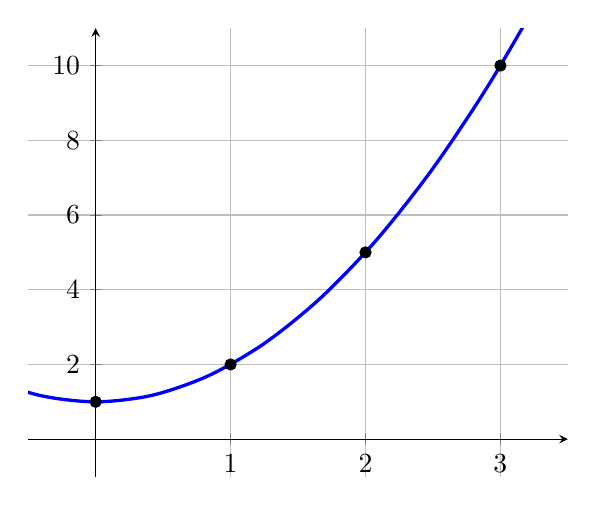
\begin{tikzpicture}
            \begin{axis}[axis lines=center, grid, xmin=-0.5, xmax=3.5, ymin=-1, ymax=11]
                \addplot[smooth, very thick, blue] {x^2 + 1};
                \addplot[mark=*, only marks] coordinates{(0,1)(1,2)(2,5)(3,10)};
            \end{axis}
        \end{tikzpicture}
    \end{center}
    \caption{A simple Vandermonde interpolation for the data set $S = \{(0,1) \, , \,
(1,2) \, , \, (2,5) \, , \, (3,10) \}$ resulting in the interpolating function $p(x) =
1+x^2$.}
    \label{fig:vandermonde}
\end{figure}


\begin{problem}\label{prob:vandermonde_1}
   Write a \ProgLang function that accepts a list of ordered pairs (where each $x$ value is
   unique) and builds a Vandermonde interpolation polynomial.  Test your function on the
   simple example listed above and then on several larger problems.  It may be simplest to
   initially test on functions that we know.
\end{problem}

\begin{problem}
    Build a Vandermonde interpolation polynomial to interpolate the function $f(x) =
    \cos(2 \pi x)$ with 10 points that are linearly spaced on the interval $x \in [0,2]$.
\end{problem}

\begin{definition}[The Vandermonde Matrix]
    Let $S = \{(x_0,y_0) \,,\, (x_1,y_1) \,,\, \ldots, (x_n,y_n)\}$ be a list of ordered
    pairs where the $x$ values are all unique.  Using Vandermonde interpolation we arrive
    at the system of equations
    \begin{flalign}
        \begin{pmatrix} 1 & x_0 & x_0^2 & \cdots & x_0^n \\
                        1 & x_1 & x_1^2 & \cdots & x_1^n \\
                        1 & x_2 & x_2^2 & \cdots & x_2^n \\
                        \vdots & \vdots & \vdots & \ddots & \vdots \\
                        1 & x_n & x_n^2 & \cdots & x_n^n \end{pmatrix}
        \begin{pmatrix} \beta_0 \\ \beta_1 \\ \beta_2 \\ \vdots \\ \beta_n \end{pmatrix}
        =
        \begin{pmatrix} y_0 \\ y_1 \\ y_2 \\ \vdots \\ y_n \end{pmatrix}.
        \label{eqn:vandermonde}
    \end{flalign}
    The matrix on the left-hand side of \eqref{eqn:vandermonde} is called the {\bf
    Vandermonde Matrix}.
\end{definition}

\begin{problem}
    Vandermonde matrix is relatively easy to conceptualize and code, but there is an
    inherent problem.  Use your code from Problem \ref{prob:vandermonde_1} to create a
    plot on a \mcode{semilogy} scale.  The horizontal axis of the plot is the order of the
    interpolating polynomial and the vertical axis is the ratio
    $|\lambda_{max}|/|\lambda_{min}|$ where $\lambda_{max}$ and $\lambda_{min}$ are the
    maximum and minimum eigenvalues of the Vandermonde matrix respectively.  What does
    this plot tell you about Vandermonde interpolation for high-order polynomials?
\end{problem}

\subsection{Lagrange Interpolation}
Lagrange interpolation is a rather clever interpolation scheme where we build up the
polynomial from simpler polynomials.  For interpolation we want to build a polynomial
$p(x)$ such that $p(x_j) = y_j$.  If we can find a polynomial $\phi_j(x)$ that 
\[ \phi_j(x) = \left\{ \begin{array}{ll} 0, & \text{ if } x = x_i \text{ and } i \ne j \\ 1, & \text{ if
    } x=x_j \end{array} \right. \]
then for Lagrange interpolation we build $p(x)$ as a linear combination of the $\phi_j$ functions.

\begin{problem}
    Consider the data set $S = \{(0,1) \, , \, (1,2) \, , \, (2,5) \, , \, (3,10) \}$.
    
    \begin{enumerate}
        \item[(a)] Based on the descriptions of the $p(x)$ and $\phi_j(x)$ functions, why would
            $p(x)$ be defined as
            \[ p(x) = 1 \phi_0(x) + 2 \phi_1(x) + 5 \phi_2(x) + 10 \phi_3(x)? \]
        \item[(b)] Verify that $\phi_0(x)$ can be defined as
            \[ \phi_0(x) = \frac{(x-1)(x-2)(x-3)}{(0-1)(0-2)(0-3)}. \]
        \item[(c)] Verify that $\phi_1(x)$ can be defined as
            \[ \phi_1(x) = \frac{(x-0)(x-2)(x-3)}{(1-0)(1-2)(1-3)}. \]
        \item[(d)] Define $\phi_2(x)$ and $\phi_3(x)$ in a similar way.
        \item[(e)] Build the linear combination from part (a) and create a plot showing that
            this polynomial indeed interpolates the points in the set $S$.
    \end{enumerate}
\end{problem}

\begin{technique}[Lagrange Interpolation]
    To build an interpolating polynomial $p(x)$ for the set of points
    $\{(x_0,y_0)\,,\,(x_1,y_1)\,,\,(x_2,y_2)\,,\ldots,\,(x_n,y_n)\}$ we first build the
    polynomials $\phi_j(x)$ for each $j = 0, 1, 2, \ldots, n$ and then construct the
    polynomial $p(x)$ as 
    \[ p(x) = \sum_{j=0}^n y_j \phi_j(x). \]
    The $\phi_j(x)$ functions are defined as
    \[ \phi_j(x) = \prod_{i \ne j} \frac{x-x_i}{x_j-x_i}. \]
\end{technique}

\begin{example}
    Build a Lagrange interpolation polynomial for the set of points
    \[ S  = \{(1,5)\,,\,(2,9)\,,\,(3,11)\}. \]
    {\bf Solution} \\
    We first build the three $\phi_j$ functions.
    \begin{flalign*}
        \phi_0(x) = \frac{(x-2)(x-3)}{(1-2)(1-3)} \\
        \phi_1(x) = \frac{(x-1)(x-3)}{(2-1)(2-3)} \\
        \phi_2(x) = \frac{(x-1)(x-2)}{(3-1)(3-2)}.
    \end{flalign*}
    Take careful note that the $\phi$ functions are built in a very particular way.
    Indeed, $\phi_0(1) = 1$, $\phi_0(2) =0$, and $\phi_0(3) = 0$.  Also, $\phi_1(1) = 0$,
    $\phi_1(2) = 1)$, and $\phi_1(3) = 0$.  Finally, note that $\phi_2(1) = 0$, $\phi_2(1)
    = 0$ and $\phi_2(3) = 1$.  Thus, the polynomial $p(x)$ can be built as
    \[ p(x) = 5 \phi_0(x) + 9 \phi_1(x) + 11 \phi(2(x) = 5 \frac{(x-2)(x-3)}{(1-2)(1-3)} +
    \frac{(x-1)(x-3)}{(2-1)(2-3)} + \frac{(x-1)(x-2)}{(3-1)(3-2)}. \]
    The remainder of the simplification is left to the reader.
\end{example}

\begin{problem}
    Write a \ProgLang function that accepts a list of list of ordered pairs (where each $x$
    value is unique) and builds a Lagrange interpolation polynomial.  Test your function
    on the examples that we've presented in this section.
\end{problem}

\subsection{Interpolation at Chebyshev Points}
\begin{problem}
    Using either Vandermonde or Lagrange interpolation build a polynomial that
    interpolates the function 
    \[ f(x) = \frac{1}{1+x^2} \]
    for $x \in [-5,5]$
    with polynomials of order $n=2, 3, \ldots$ and linearly spaced interpolation
    points.  What do you notice about the
    quality of the interpolating polynomial near the endpoints?
    \begin{center}
        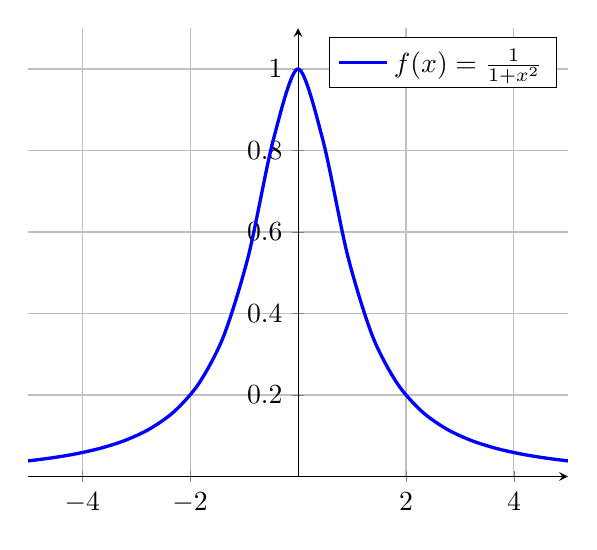
\begin{tikzpicture}
            \begin{axis}[axis lines=center, grid, domain=-5.5:5.5, xmin=-5, xmax=5,
                ymin=0, ymax=1.1] 
                \addplot[smooth, very thick, blue] {1/(1+x^2)};
                \addlegendentry{$f(x) = \frac{1}{1+x^2}$};
            \end{axis}
        \end{tikzpicture}
    \end{center}
\end{problem}

As you should have noticed the quality of the interpolation gets rather terrible near the
endpoints when you use linearly spaced points for the interpolation.  A fix to this was
first proposed by the Russian mathematician Pafnuty Chebyshev (1821-1894).  The idea is as
follows:
\begin{itemize}
    \item Draw a semicircle above the closed interval on which you are interpolating
        (shown in black in Figure \ref{fig:chebyshev_nodes}).
    \item Pick $n$ equally spaced points along the semicircle (i.e. same arc length between
        each point).  (shown in blue in Figure \ref{fig:chebyshev_nodes})
    \item Project the points on the semicircle down to the interval.  Use these projected
        points for the interpolation. (shown in red in Figure \ref{fig:chebyshev_nodes})
\end{itemize}

\begin{figure}
    \begin{center}
        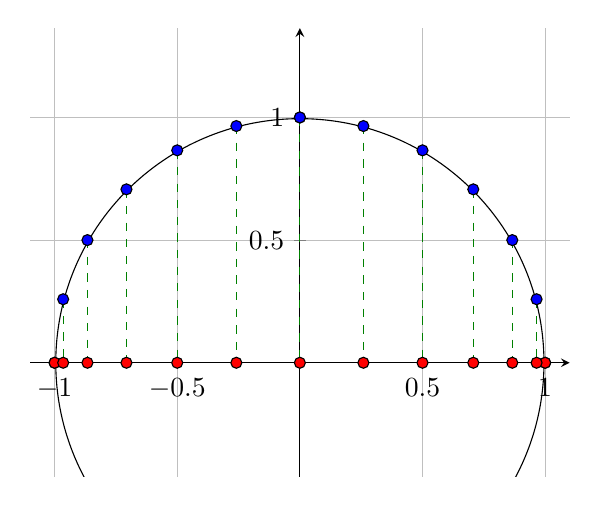
\begin{tikzpicture}
            \begin{axis}[axis equal, axis lines=center, xmin=-1.1, xmax=1.1, ymin=-0.2, ymax=1.1,
                grid]
%                 \addplot[smooth, very thick, samples=200] {sqrt(1-x^2)};
                %
                \draw[dashed, color=green!50!black] (axis cs:1,0) -- (axis cs:1,0);
                \draw[dashed, color=green!50!black] (axis cs:0.965,0.259) -- (axis cs:0.965,0);
                \draw[dashed, color=green!50!black] (axis cs:0.866,0.5) -- (axis cs:0.866,0);
                \draw[dashed, color=green!50!black] (axis cs:0.707,0.707) -- (axis cs:0.707,0);
                \draw[dashed, color=green!50!black] (axis cs:0.5,0.866) -- (axis cs:0.5,0);
                \draw[dashed, color=green!50!black] (axis cs:0.259,0.965) -- (axis cs:0.259,0);
                \draw[dashed, color=green!50!black] (axis cs:0,1) -- (axis cs:0,0);
                \draw[dashed, color=green!50!black] (axis cs:-1,0) -- (axis cs:-1,0);
                \draw[dashed, color=green!50!black] (axis cs:-0.965,0.259) -- (axis cs:-0.965,0);
                \draw[dashed, color=green!50!black] (axis cs:-0.866,0.5) -- (axis cs:-0.866,0);
                \draw[dashed, color=green!50!black] (axis cs:-0.707,0.707) -- (axis cs:-0.707,0);
                \draw[dashed, color=green!50!black] (axis cs:-0.5,0.866) -- (axis cs:-0.5,0);
                \draw[dashed, color=green!50!black] (axis cs:-0.259,0.965) -- (axis cs:-0.259,0);
                \draw[dashed, color=green!50!black] (axis cs:-0,1) -- (axis cs:-0,0);
                %
                \draw[black] (axis cs:0,0) circle(3.1cm);
                \draw[fill=blue] (axis cs:1,0) circle(0.07cm);
                \draw[fill=blue] (axis cs:0.965,0.259) circle(0.07cm);
                \draw[fill=blue] (axis cs:0.866,0.5) circle(0.07cm);
                \draw[fill=blue] (axis cs:0.707,0.707) circle(0.07cm);
                \draw[fill=blue] (axis cs:0.5,0.866) circle(0.07cm);
                \draw[fill=blue] (axis cs:0.259,0.965) circle(0.07cm);
                \draw[fill=blue] (axis cs:0,1) circle(0.07cm);
                \draw[fill=blue] (axis cs:-1,0) circle(0.07cm);
                \draw[fill=blue] (axis cs:-0.965,0.259) circle(0.07cm);
                \draw[fill=blue] (axis cs:-0.866,0.5) circle(0.07cm);
                \draw[fill=blue] (axis cs:-0.707,0.707) circle(0.07cm);
                \draw[fill=blue] (axis cs:-0.5,0.866) circle(0.07cm);
                \draw[fill=blue] (axis cs:-0.259,0.965) circle(0.07cm);
                \draw[fill=blue] (axis cs:-0,1) circle(0.07cm);
                %
                \draw[fill=red] (axis cs:1,0) circle(0.07cm);
                \draw[fill=red] (axis cs:0.965,0) circle(0.07cm);
                \draw[fill=red] (axis cs:0.866,0) circle(0.07cm);
                \draw[fill=red] (axis cs:0.707,0) circle(0.07cm);
                \draw[fill=red] (axis cs:0.5,0) circle(0.07cm);
                \draw[fill=red] (axis cs:0.259,0) circle(0.07cm);
                \draw[fill=red] (axis cs:0,0) circle(0.07cm);
                \draw[fill=red] (axis cs:-1,0) circle(0.07cm);
                \draw[fill=red] (axis cs:-0.965,0) circle(0.07cm);
                \draw[fill=red] (axis cs:-0.866,0) circle(0.07cm);
                \draw[fill=red] (axis cs:-0.707,0) circle(0.07cm);
                \draw[fill=red] (axis cs:-0.5,0) circle(0.07cm);
                \draw[fill=red] (axis cs:-0.259,0) circle(0.07cm);
            \end{axis}
        \end{tikzpicture}
    \end{center}
    \caption{Chebyshev interpolation nodes for the interval $[-1,1]$. In this case each
    node is separated by $\pi/8$ radians giving 13 interpolations points including the
endpoints.}
    \label{fig:chebyshev_nodes}
\end{figure}

It should be clear that since we are projecting down to the $x$-axis from a circle then
all we need are the cosine values from the circle.  Hence we can form the Chebyshev
interpolation points from the formula
\begin{flalign}
    x_j = \cos\left( \frac{\pi j}{n} \right), \quad \text{for} \quad j=0, 1, \ldots, n
    \label{eqn:chebyshev_cosine}
\end{flalign}
on the interval $[-1,1]$.  

To transform the Chebyshev points from the interval $[-1,1]$ (found with
\eqref{eqn:chebyshev_cosine}) to the interval $[a,b]$ we can apply a linear function which
maps $-1$ to $a$ and $1$ to $b$:
\[ x_j \gets \left( \frac{b-a}{2} \right)\left( x_j + 1 \right) + a \]
where the ``$x_j$'' on the left is on the interval $[a,b]$ and the ``$x_j$'' on the right
is on the interval $[-1,1]$.

\begin{problem}
    Consider the function $f(x) = \frac{1}{1+x^2}$ just as we did for the first problem in
    this subsection.  Write code that overlays an interpolation with linearly spaced
    points an interpolation with Chebyshev nodes.  Give plots for polynomial of order
    $n=2,3, 4, \ldots$.  Be sure to show the original function on your plots as well.
\end{problem}

\begin{problem}
    Demonstrate that the Chebyshev interpolation nodes will improve the stability of the
    Vandermonde matrix over using linearly spaced nodes.
\end{problem}




\newpage\section{Multi-Dimensional Newton's Method}\label{sec:mv_newton}
Now that we know some linear algebra let's return to the Newton's Method root finding
technique from earlier in the book. This time we will consider root finding problems where
we are not just solving the equation $f(x) = 0$ as we did Chapter
\ref{ch:numerical_algebra}.  Instead consider the function $F$ that takes a vector of
variables in and outputs a vector.  An example of such a function is
\[ F(x,y) = \begin{pmatrix} x\sin(y) \\ \cos(x) + \sin(y^2)
\end{pmatrix}. \]
It should be clear that making a picture of this type of function is a frivolous endeavor!
In the case of the previous example, there are two inputs and two outputs so the
``picture'' would have to be four dimensional.  Even so, we can still ask the question:
\begin{quote}
    {\it For what values of $x$ and $y$ does the function $F$ give the zero vector?}
\end{quote}
That is, what if we have $F$ defined as 
\[ F(x,y) = \begin{pmatrix} f(x,y) \\ g(x,y) \end{pmatrix} \]
and want to solve the system of equations
\begin{flalign*}
    f(x,y) &= 0 \\ 
    g(x,y) &= 0. 
\end{flalign*}
In the present problem this amounts to solving the nonlinear system of equations
\begin{flalign*}
    x\sin(y) &= 0 \\
    \cos(x) + \sin(y^2) &=0.
\end{flalign*}
In this case it should be clear that we are implicitly defining $f(x,y) = x\sin(y)$ and
$g(x,y) = \cos(x) + \sin(y^2)$.  A moment's reflection (or perhaps some deep meditation)
should reveal that $(\pm\pi/2,0)$ are two solutions to the system, and given the trig
functions it stands to reason that $(\pi/2 + \pi k,\pi j)$ will be a solution for all
integer values of $k$ and $j$.

\begin{problem}
To build a numerical solver for a nonlinear system of equations, let's just recall
Newton's Method in one dimension and then mimic that for systems of higher dimensions.
We'll stick to two dimensions in this problem for relative simplicity.
\begin{enumerate}
    \item[(a)] In Newton's Method we first found the derivative of our function.  In a
        nonlinear system such as this one, talking about ``the derivative'' is a bit
        nonsense since there are many first derivatives.  Instead we will define the
        Jacobian matrix $J(x,y)$ as a matrix of the first partial derivatives of the
        functions $f$ and $g$.
        \[ J(x,y) = \begin{pmatrix} f_x & f_y \\ g_x & g_y \end{pmatrix}. \]
        In the present example (fill in the rest of the blanks),
        \[ J(x,y) = \begin{pmatrix} \sin(y) &
                \underline{\hspace{0.5in}} \\  \underline{\hspace{0.5in}} &
            \underline{\hspace{0.5in}} \end{pmatrix}. \]
    \item[(b)] Now let's do some Calculus and algebra.  Your job in this part of this
        problem is to follow all of the algebraic steps.
        \begin{enumerate}
            \item[(i)] In one-dimensional Newton's Method we then write the equation of a tangent
        line at a point $(x_0, f(x_0))$
        \[ f(x) - f(x_0) \approx f'(x_0)(x-x_0) \]
        to give a local approximation to the function.  
        We'll do the exact same thing here, but in place of ``$x$'' we need to have a
        vector and in place of the derivative we need to have the Jacobian
        \[ F(x,y) - F(x_0,y_0) \approx J(x_0, y_0) \left( \begin{pmatrix} x \\ y
        \end{pmatrix} - \begin{pmatrix} x_0 \\ y_0 \end{pmatrix} \right). \]
%         Write this equation in vector form for the functions $f(x,y) = x\sin(y)$ and
%         $g(x,y) = \cos(x) + \sin(y^2)$.
    \item[(ii)] In one-dimensional Newton's Method we then set $f(x)$ to zero since we were
        ultimately trying to solve the equation $f(x) = 0$.  Hence we got the equation 
        \[ 0 - f(x_0) \approx f'(x_0)(x-x_0) \]
        and then rearranged to solve for $x$.  This gave us 
        \[ x \approx x_0 - \frac{f(x_0)}{f'(x_0)}. \]
        In the multi-dimensional case we have the same goal.  If we set $F(x,y)$ to the
        zero vector and solve for the vector $\begin{pmatrix}x\\y\end{pmatrix}$ then we
        get
        \[ \begin{pmatrix} x\\y\end{pmatrix} \approx \begin{pmatrix}
                x_0 \\ y_0 \end{pmatrix} -
            \left[ J(x_0,y_0) \right]^{-1} F(x_0,y_0). \]
        Take very careful note here that we didn't divide by the Jacobian \ldots it is a
        matrix after all!!
        \item[(iii)] The final step in one-dimensional Newton's Method was to turn the
            approximation of $x$ into an iterative process by replacing $x$ with $x_{n+1}$ and
            replacing $x_0$ with $x_{n}$ resulting in the iterative form of Newton's
            Method
            \[ x_{n+1} = x_{n} - \frac{f(x_n)}{f'(x_n)}. \]
            We can do the exact same thing in the two-dimensional version of Newton's
            Method to arrive at 
            \[ \boxed{ \begin{pmatrix} x_{n+1} \\ y_{n+1} \end{pmatrix} = \begin{pmatrix}
            x_n \\ y_n \end{pmatrix} - J^{-1}(x_n,y_n) F(x_n, y_n).} \]
        Writing this in full matrix-vector form we get
            \[ \boxed{ \begin{pmatrix} x_{n+1} \\ y_{n+1} \end{pmatrix} = \begin{pmatrix}
                x_n \\ y_n \end{pmatrix} - \begin{pmatrix} f_x & f_y \\ g_x & g_y
        \end{pmatrix}^{-1} \begin{pmatrix} f(x_n,y_n) \\ g(x_n,y_n) \end{pmatrix}.} \]
\end{enumerate}
\item[(c)] Write down the Newton iteration formula for the system
    \begin{flalign*}
        x\sin(y) &= 0 \\
        \cos(x) + \sin(y^2) &= 0.
    \end{flalign*}
    Do not actually compute the matrix inverse of the Jacobian.
\item[(d)] The inverse of the Jacobian needs to be dealt with carefully.  We typically
    don't calculate inverses directly in numerical analysis, but since we have some other
    tools to do the work we can think of it as follows:
    \begin{itemize}
        \item We need the vector $\bb = J^{-1}(x_n,y_n) F(x_n,y_n)$.
        \item The vector $\bb$ is the same as the solution to the equation $J(x_n,y_n) \bb
            = F(x_n,y_n)$ at each iteration of Newton's Method.
        \item Therefore we can so a relatively fast linear solve (using any technique from
            this chapter) to find $\bb$.
        \item The Newton iteration becomes 
            \[ \begin{pmatrix} x_{n+1} \\ y_{n+1} \end{pmatrix} = \begin{pmatrix} x_n \\
                y_n \end{pmatrix} - \bb. \]
    \end{itemize}
    Write code to solve the present nonlinear system of equations.  Implement some sort of
    linear solver within your code and be able to defend your technique.  Be prepared to
    share your answer and your technique with your peers.  Try to pick a starting point so
    that you find the solution $(\pi/2,\pi)$ on your first attempt at solving this
    problem.  Then play with the starting point to verify that you can get the other
    solutions.
\end{enumerate}
\end{problem}



\begin{problem}
    Test your code from the previous problem on the system of nonlinear equations
    \begin{flalign*}
        1+x^2 - y^2 + e^x\cos(y) &= 0 \\
        2xy + e^x\sin(y) &=0.
    \end{flalign*}
    Note here that $f(x,y) = 1+x^2 - y^2 + e^x\cos(y)$ and $g(x,y) = 2xy + e^x \sin(y)$.
\end{problem}



\begin{problem}\label{prob:mv_newton}
    Let's generalize the process a bit so we can numerically approximate solutions to systems of nonlinear algebraic
    equations in any number of dimensions.
    The Newton's method that we derived in Chapter \ref{ch:numerical_algebra} is only
    applicable to functions $f: \mathbb{R} \to \mathbb{R}$ (functions mapping a real
    number to a real number).   In the previous problem we build a method for solving the
    equation $F(x,y) = (0,0)$ where $F: \mathbb{R}^2 \to \mathbb{R}^2$.  What about
    vector-valued functions in $n$ dimensions?  In particular, we
    would like to have an analogous method for finding roots of a function $F$ where $F:
    \mathbb{R}^k \to \mathbb{R}^k$.

    Let $\bx$ be a vector in $\mathbb{R}^k$, let 
    \[ F(\bx) = \begin{pmatrix} f_1(\bx) \\ f_2(\bx) \\ \vdots \\ f_k(\bx) \end{pmatrix} \]
    be a vector valued function, and let $J$ be the Jacobian matrix
    \[ J(\bx) = 
        \begin{pmatrix} \partial f_1 / \partial x_1(\bx) & \partial f_1 / \partial
            x_2(\bx) & \cdots
            & \partial f_1 / \partial x_k(\bx) \\ 
         \partial f_2 / \partial x_1(\bx) & \partial f_2 / \partial x_2(\bx) & \cdots &
         \partial f_2 / \partial x_k(\bx) \\ 
         \vdots & \vdots & \ddots & \vdots \\
         \partial f_k / \partial x_1(\bx) & \partial f_k / \partial x_2(\bx) & \cdots & \partial f_k /
     \partial x_k(\bx) \end{pmatrix} \]
    By analogy, the multi-dimensional Newton's method is
    \[ \bx_{n+1} = \bx_n -  J^{-1}(\bx_n)F(\bx_n) \]
    where $J^{-1}(\bx_n)$ is the inverse of the Jacobian matrix evaluated at the point
    $\bx_n$.
    \begin{enumerate}
        \item[(a)] Write code that accepts any number of functions and an initial
            vector guess and returns an approximation to the root for the problem $F(\bx) = \bo$.
        \item[(c)] Use Newton's method to find an approximate solution to the system of
            equations
            \begin{flalign*}
                x^2 + y^2 + z^2 &= 100 \\
                xyz &= 1 \\
                x - y - \sin(z) &= 0
            \end{flalign*}
    \end{enumerate}
\end{problem}
% \hint{
%     If you want to evaluate the matrix-vector multiplication $J^{-1}(\bx_n) F(\bx_n)$ then
%     you are really looking for the solution $\bu$ to the system of equations $J(\bx_n) \bu =
%     F(\bx_n)$ and you can use MATLAB's backslash command to get it quickly. 
% 
%     For part (c) be sure to first make the right-hand side zero.
% }

\begin{technique}[Multi-Dimensional Newton's Method]
    The iteration for Newton's Method in multiple dimensions is
    \[ \bx_{n+1} = \bx_n - J^{-1}(\bx_n) F(\bx_n) \]
    where $\bx_n \in \mathbb{R}^k$, $J$ is the $k$-dimensional Jacobian matrix, and
    $F:\mathbb{R}^k \to \mathbb{R}^k$.  Take note that numerically you do not want to
    directly compute the inverse of the Jacobian.  Instead you solve the sub-problem
    \[ J(\bx_n) \bb = F(\bx_n) \]
    for the vector $\bb$ using any technique from linear algebra (e.g. an LU or QR
    decomposition) and iterate the equation
    \[ \bx_{n+1} = \bx_n - \bb. \]
\end{technique}


\begin{problem}
    When will the multi-dimensional version of Newton's Method fail?  Compare and contrast
    this with what you found about the one-dimensional version of Newton's Method in
    Chapter \ref{ch:numerical_algebra}.  Extend your discussion to talk about the
    eigenvalues of the Jacobian matrix for a nonlinear system.
\end{problem}

One place that solving nonlinear systems arises naturally is when we need to find
equilibrium points for systems of differential equations.  Remember that to find the
equilibrium points for a first order differential equation we set the derivative term to
zero and solve the resulting equation.  
\begin{problem}
    Find the equilibrium point(s) for the system of differential equations 
    \begin{flalign*}
        x' &= \alpha x - \beta xy \\
        y' &= \delta y + \gamma xy
    \end{flalign*}
    where $\alpha = 1, \beta = 0.05, \gamma = 0.01$ and $\delta =1$.  You will play more
    with this differential equation system later.
\end{problem}



\begin{problem}
    Find the equilibrium point(s) for the system of differential equations
    \begin{flalign*}
        x' &= -0.1 xy - x \\
        y' &= -x + 0.9y \\
        z' &= \cos(y) - xz
    \end{flalign*}
    if they exist.
\end{problem}



\begin{problem}\label{prob:lawn_chair}
    (This problem is modified from \cite{Meerschaert}) \\
    A manufacturer of lawn furniture makes two types of lawn chairs, one with a wood
    frame and one with a tubular aluminum frame.  The wood-frame model costs \
    418 per unit to manufacture, and the aluminum-frame model costs \$10 per unit.  The
    company operates in a market where the number of units that can be sold depends on the
    price.  It is estimated that in order to sell $x$ units per day of the wood-frame
    model and $y$ units per day of the aluminum-frame model, the selling price cannot
    exceed 
    \[ 10 + \frac{31}{\sqrt{x}} + \frac{1.3}{y^{0.2}} \text{ dollars per unit} \]
    for wood-frame chairs, and 
    \[ 5 + \frac{15}{y^{0.4}} + \frac{0.8}{x^{0.08}} \text{ dollars per unit} \]
    for the aluminum chairs.  We want to find the optimal production levels.  Write this
    situation as a multi-variable mathematical model, use a computer
    algebra system (or by-hand computation) to find the gradient vector, and then use the
    multi-variable Newton's method to find the critical points.  Classify the critical
    points as either local maximums or local minimums.
\end{problem}



\newpage\section{Building PDE's From Conservation Laws}

In this section
we'll give a more analytic introduction to most of the primary partial
differential equations of interest in basic mathematical physics.  We will make reference
to Fick's Law for mass transport and Fourier's Law for thermal transport, so interested
readers should dig deeper by examining the relevant Wikipedia pages or other sources.
  
Conservation laws pervade all of physics -- conservation of energy, conservation of
momentum, and conservation of mass.  These laws are sometimes stated colloquially as
{\it energy (or momentum or mass) can neither be created nor destroyed}, but this phrase
is not super helpful mathematically.  We start this section with a brief mathematical
derivation of a {\it general conservation law} to further clarify what we mean
mathematically.  The resulting general conservation law will be a
partial differential equation that can be used to mathematically express the physical laws
of conservation of mass, momentum, or
energy.

Let $u$ be the quantity you are trying to conserve, $\bq$ be the flux of that quantity,
and $f$ be any source of that quantity.  For example, if we are to derive a conservation
of energy equation, $u$ might be energy, $\bq$ might be temperature flux, and $f$ might be
a temperature source (or sink).

\subsection*{Derivation of General Balance Law}
Let $\Omega$ be a fixed volume and denote the boundary of this volume by $\partial
\Omega$. The rate at which $u$ is changing in time throughout $\Omega$ needs to be
balanced by the rate at which $u$ leaves the volume plus any sources of $u$.
Mathematically, this means that
\begin{flalign}
    \pd{ }{t} \iiint_{\Omega} u dV = -\iint_{\partial \Omega} \bq \cdot n dA +
    \iiint_\Omega f dV.
    \label{eqn:global_balance}
\end{flalign}
This is a global balance law in the sense that it holds for all volumes $\Omega$.  The
mathematical 
troubles here are two fold: (1) there are many integrals, and (2) there are really two variables
($u$ and $q$ since $f=f(u,x,t)$) so the equation is not closed.  In order to mitigate
that fact we apply the divergence theorem to the first term on the right-hand side of
\eqref{eqn:global_balance} to get
\begin{flalign}
    \pd{ }{t} \iiint_{\Omega} u dV = -\iiint_{\Omega} \nabla \cdot \bq dV +
    \iiint_\Omega f dV.
    \label{eqn:global_balance2}
\end{flalign}

Gathering all of the terms on the right of \eqref{eqn:global_balance2}, interchanging the integral and the derivative on
the left (since the volume is not changing in time), and rewriting gives
\begin{flalign}
    \iiint_\Omega \left( \pd{u}{t} + \nabla \cdot \bq \right) dV = \iiint_\Omega f dV
    \label{eqn:global_balance3}
\end{flalign}
If we presume that this equation holds for all volumes $\Omega$ then the integrands must
be equal and we get the local balance law
\begin{flalign}
    \pd{u}{t} + \nabla \cdot \bq = f.
    \label{eqn:local_balance}
\end{flalign}

Equation \eqref{eqn:local_balance} is an expression of the balances of changes in time to
changes in space of a conserved quantity such as mass, momentum, or energy.  What remains
is to make clear the meaning and functional form of the flux $\bq$ and the source function
$f$.

\subsection*{Simplification of the Local Balance Law}
In equation \eqref{eqn:local_balance} it is often assumed that the system is free of
external sources.  In this case we set $f$ to zero and obtain the source-free balance law
\begin{flalign}
    \pd{u}{t} + \nabla \cdot \bq = 0.
    \label{eqn:local_source_free}
\end{flalign}
It is this form of balance law where many of the most interesting and important partial
differential equations come from.  In particular consider the following two cases: mass
balance and energy balance.
\subsection*{Mass Balance}
In mass balance we take $u$ to either be the density of a substance (e.g. in the case of
liquids) or the concentration of a substance in a mixture (e.g. in the case of
gasses). If $C$ is the mass concentration of a substance in a gas then the flux of that
substance is given via Fick's Law as
\begin{flalign}
    \bq = -k \nabla C.
    \label{eqn:fick}
\end{flalign}
Combining \eqref{eqn:fick} with \eqref{eqn:local_source_free} (and assuming that $k$ is
independent of space, time, and concentration) gives
\begin{flalign}
    \pd{C}{t} = k \nabla \cdot \nabla C. 
    \label{eqn:fick2_simp}
\end{flalign}
In the presence of external sources of mass, \eqref{eqn:fick2_simp} is
\begin{flalign}
    \pd{C}{t} = k \nabla \cdot \nabla C + f(x).
    \label{eqn:fick3}
\end{flalign}
Expanding the Laplacian operator on the right-hand side of \eqref{eqn:fick3} we get
\begin{flalign}
    \pd{C}{t} = k\left( \pdd{C}{x} + \pdd{C}{y} + \pdd{C}{z} \right) + f(x)
    \label{eqn:fick3_expanded}
\end{flalign}
where the reader should note that this can be easily simplified in 1 or 2 spatial
dimensions.
% \begin{problem}
%     What does \eqref{eqn:fick3} equation look like in terms of spatial derivatives on the
%     right-hand side?
%     \begin{flalign*}
%         \pd{C}{t} &= \underline{\hspace{2in}} \quad \text{(1 Spatial Dimension)} \\
%         \pd{C}{t} &= \underline{\hspace{2in}} \quad \text{(2 Spatial Dimensions)} \\
%         \pd{C}{t} &= \underline{\hspace{2in}} \quad \text{(3 Spatial Dimensions)}
%     \end{flalign*}
% \end{problem}

\subsection*{Energy Balance}
The energy balance equation is essentially the same as the mass balance equation.  If $u$
is temperature then the flux of temperature is given by Fourier's Law for heat conduction
\begin{flalign}
    \bq = -k\nabla T.
    \label{eqn:fourier}
\end{flalign}
Making the same simplifications as in the mass balance equation we arrive at
\begin{flalign}
    \pd{T}{t} = k \nabla \cdot \nabla T.
    \label{eqn:fourier2}
\end{flalign}
In the presence of external sources of heat, \eqref{eqn:fourier2} becomes
\begin{flalign}
    \pd{T}{t} = k \nabla \cdot \nabla T + f(x).
    \label{eqn:fourier3}
\end{flalign}
Expanding the Laplacian operator on the right-hand side of \eqref{eqn:fourier3} we get
\begin{flalign}
    \pd{T}{t} = k\left( \pdd{T}{x} + \pdd{T}{y} + \pdd{T}{z} \right) + f(x)
    \label{eqn:fourier3_expanded}
\end{flalign}
where the reader should note that this can be easily simplified in 1 or 2 spatial
dimensions.
% \begin{problem}
%     What does \eqref{eqn:fourier3} equation look like in terms of spatial derivatives on the
%     right-hand side?
%     \begin{flalign*}
%         \pd{T}{t} &= \underline{\hspace{2in}} \quad \text{(1 Spatial Dimension)} \\
%         \pd{T}{t} &= \underline{\hspace{2in}} \quad \text{(2 Spatial Dimensions)}\\
%         \pd{T}{t} &= \underline{\hspace{2in}} \quad \text{(3 Spatial Dimensions)}
%     \end{flalign*}
% \end{problem}



\subsection*{Laplace's Equation and Poisson's Equation}
Equations \eqref{eqn:fick3} and \eqref{eqn:fourier3} are the same partial differential
equation for two very important physical phenomenon; mass and heat transfer.  In the case
where time is allowed to run to infinity and no external sources of mass or energy are
included these equations reach a steady state solution (no longer changing in time) and we
arrive at Laplace's Equation
\begin{flalign}
    \nabla \cdot \nabla u = 0.
    \label{eqn:laplace}
\end{flalign}
Laplace's equation is actually a statement of minimal energy as well as steady state heat
or temperature.  We can see this since entropy always drives systems from high energy to
low energy, and if we have reached a steady state then we must have also reached a surface
of minimal energy.

Equation \eqref{eqn:laplace} is sometimes denoted as $\nabla \cdot \nabla u = \nabla^2 u =
\Delta u$, and in terms of the partial derivatives it is written as
\begin{flalign*}
    \pdd{u}{x} + \pdd{u}{y} + \pdd{u}{z} = 0.
% V    0 &= \underline{\hspace{2in}} \quad \text{(1 Spatial Dimension)} \\
%     0 &= \underline{\hspace{2in}} \quad \text{(2 Spatial Dimensions)} \\
%     0 &= \underline{\hspace{2in}} \quad \text{(3 Spatial Dimensions)} 
\end{flalign*}

If there is a time-independent external source the right-hand side of
\eqref{eqn:laplace} will be non-zero and we arrive at Poisson's equation:
\begin{flalign}
    \nabla \cdot \nabla u = -f(x).
    \label{eqn:poisson}
\end{flalign}
Note that the negative on the right-hand side comes from the fact that
$\pd{u}{t} = k \nabla \cdot \nabla u + f(x)$ and $\pd{u}{t} \to 0$.  Technically we are
absorbing the constant $k$ into $f$ (that is ``$f$'' is really ``$f/k$'').  Also
note that in many instances the value of $k$ is not constant and cannot therefore be pulled
out of the derivative without a use of the product rule.

Let's summarize:
\begin{center}
    \begin{tabular}{|c|c|c|}
        \hline
        Name of PDE & PDE & What the PDE Models \\ \hline \hline
        The Heat Equation & $\ds \pd{u}{t} = k \nabla \cdot \nabla u + f(x)$ & Diffusion \\
        Laplace's Equation & $\ds k \nabla \cdot \nabla u =-f(x)$ & Minimal Energy
        Surfaces \\
%         The Wave Equation & $\ds \pdd{u}{t} = k \nabla \cdot \nabla u + f(x)$ & Wave
%         phenomena \\
        \hline
    \end{tabular}
\end{center}

Further discussion of the origins of the wave equation and other interesting PDE's is left
to the reader.

